% Document settings
\documentclass[a4paper,11pt]{article}

% Packages
  % math formulas
\usepackage{amsmath,amsthm,amssymb}
  % graphics
\usepackage{graphicx}
\usepackage{wrapfig}
  % plots
\usepackage{pgfplots}
  % other
\usepackage[warn]{mathtext}
\usepackage{cmap}
\usepackage[T1,T2A]{fontenc}
\usepackage[utf8]{inputenc}
\usepackage[english,russian]{babel}
\usepackage{icomma}

% Package settings
%% graphicx
\graphicspath{{Pictures/}}
\DeclareGraphicsExtensions{.pdf,.png,.jpg}
%% pgfplots
\pgfplotsset{width=10cm,compat=1.9}

% Title
\title{Отчет о выполнении работы №2.3.1\\Получение и измерение вакуума}
\author{Воейко Андрей Александрович, Б01--109}
\date{Долгопрудный, 2022}

% Document
\begin{document}
\maketitle
\newpage
\section{Аннотация.}
В работе регистрируется концентрация геллия и воздуха от временис помощью датчиков теплопроводности при разных начальных давлениях смеси газов. Также в ней определятеся коэффицент диффузии по резльтатам измерений.
\section{Теоретические сведения и описание установки.}
Диффузией называется самопроизвольное перемешивание молекул, происходящее вследствие их теплового движения. Соответственно, в жидкостях она происходят быстрее, чем в твердых телах, но медленне. чем в газообразных веществах. Диффузия молекул одного рода называется самодиффузией, а перемешивание разных молекул --- взаимной диффузией.\\
Для исследования взаимной диффузии газов и определения коэффицента диффузии используется установка, изображенная на рисунке~\ref{fig:img1}. Два сосуда с объемами $V_{1} = 1200 \pm 30\ см^{3}$ и $V_{2} = 1200 \pm 30\ см^{3}$ соединены трубкой длины l и сечения S, причем $l/S = 5,5 \pm 0,5\ см^{-1}$. Сосуды заполнены смесь. двух газов при одинаковом давлении, но с различной концентрацией компонентов. Вследствие взаимной диффузии концентрация компонентов в обоих сосудах с течением времени выравнивается.
\begin{figure}[h!]\label{fig:img1}
  \centering
  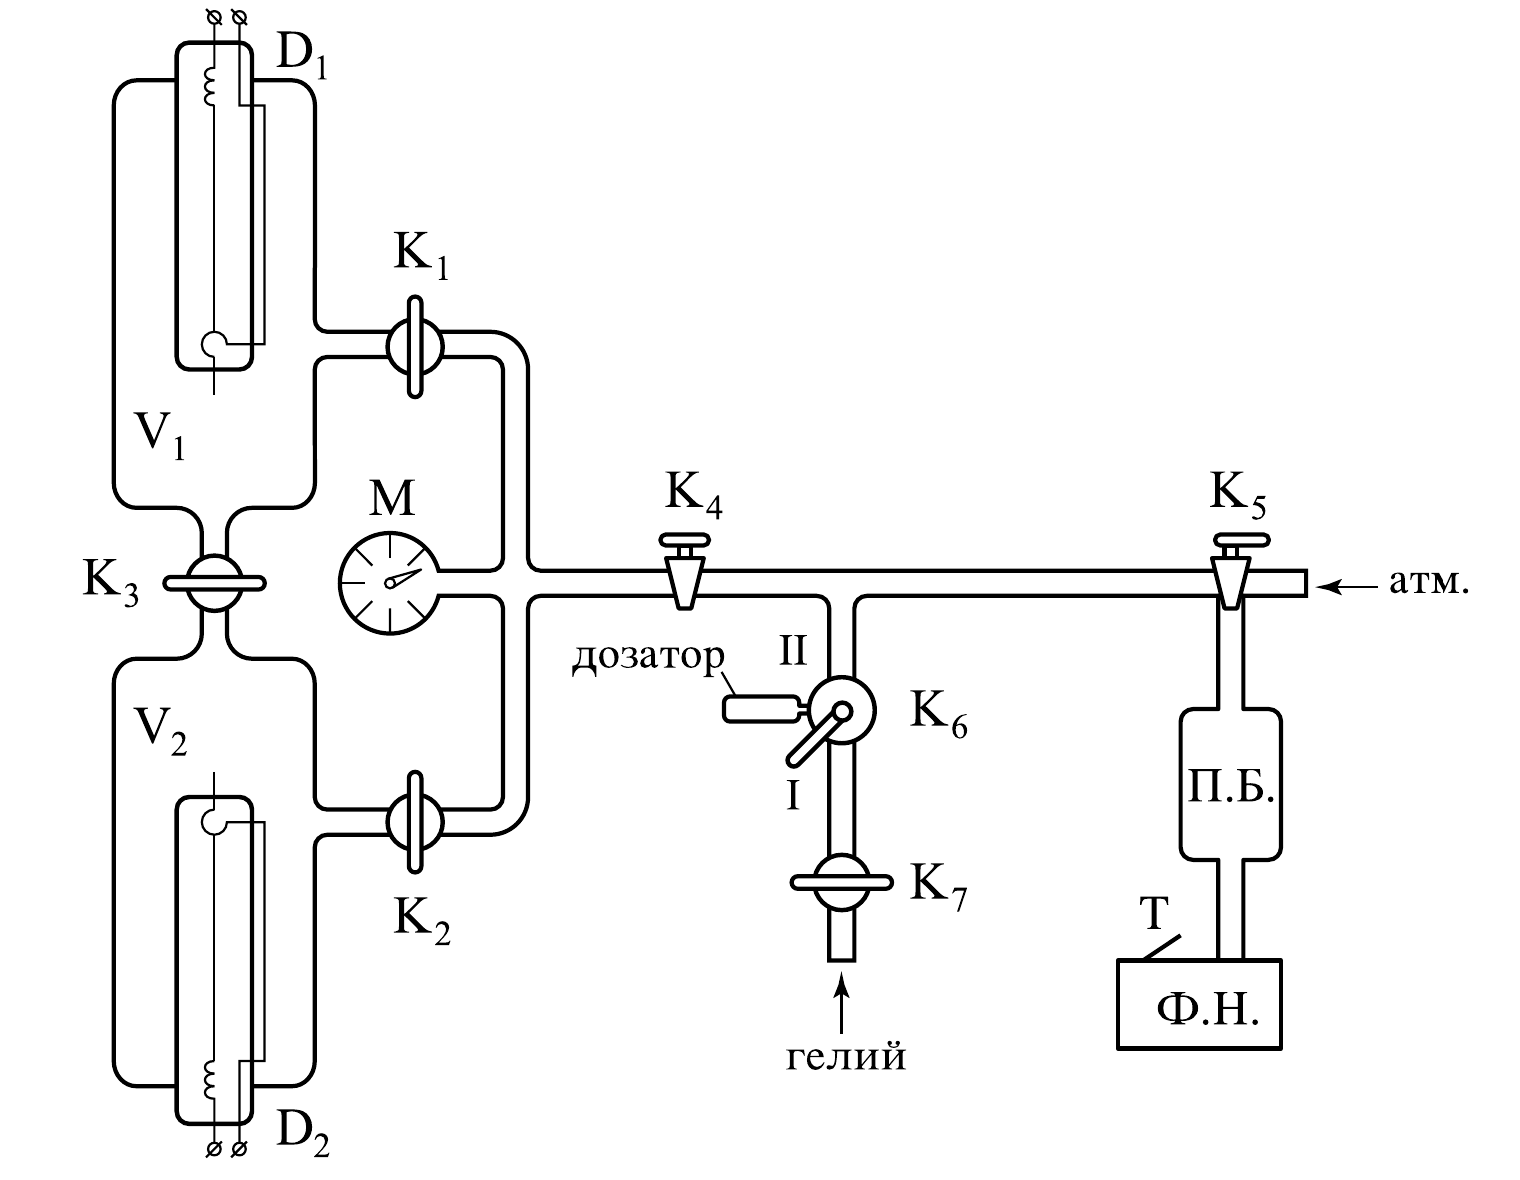
\includegraphics[scale = 0.2691]{scheme1.png}
  \caption{Схема экспериментальной установки.}
\end{figure}
Рассмотрим процесс выравнивания концентрации. Пусть концентрации одного из компонентов смеси в сосудах $V_{1}$ и $V_{2}$ равны $n_{1}$ и $n_{2}$. Плотность диффузионного потока любого компонента (т. е. количество вещества, проходящее в единицу времени через единичную поверхность) определяется законом Фика:
\begin{equation}\label{eq1}
  j = -D \frac{\delta n}{\delta x},
\end{equation}
где $D$~--- коэффицента взаимной диффузии газов, а $j$~--- плотность потока частиц. В наших условиях решение задачи упрощается благодаря тому, что объем соединительной трубки мал по сравнению с объемами сосудов, а концентрацию газов внутри каждого сосуда можно считать постоянной по всему объему. Диффузионный поток в любои сечении трубки одинаков. Поэтому $J = DS(\delta n/\delta x)$ не меняется вдоль трубки. Следовательно,
\begin{equation}\label{eq2}
  J = -DS\ \frac{n_{1} - n_{2}}{l}.
\end{equation}
Обохначим через $\Delta n_{1}$ и $\Delta n_{2}$ изменения концентрации в объемах $V_{1}$ и $V_{2}$ за время $\Delta t$. Тогда $V_{1} \Delta n_{1}$ равно измерению количества компонента в объеме $V_{1}$, а $V_{2} \Delta n_{2}$~--- измерению количества
того компонента в $V_{2}$. Из закона сохранения везества следует, что $V_{1}n_{1} + V_{2}n_{2} = $ const, откуда $V_{1} \Delta n_{1} = -V_{2} \Delta n_{2}$. Эти изменения происходят вследствие диффузии, поэтому
\begin{equation}\label{eq3}
  V_{1} \Delta n_{1} = -V_{2} \Delta n_{2} = J \Delta t = - DS\ \frac{n_{1} - n_{2}}{l} \Delta t.
\end{equation}
Деля это равенство на $\Delta t$, получаем
\begin{equation}\label{eq4}
  V_{1}\ \frac{dn_{1}}{dt} = -DS\ \frac{n_{1} - n_{2}}{l},\ \ \ \ V_{2}\ \frac{dn_{2}}{dt} = DS\ \frac{n_{1} - n_{2}}{l}.
\end{equation}
Разделив уравнения на $V_{1}$ и $V_{2}$ соответственно, и вычитая одно из другого, получаем
\begin{equation}\label{eq5}
\frac{dn_{1}}{dt} - \frac{dn_{2}}{dt} = -\frac{n_{1} - n_{2}}{l}\ DS \left(\frac{1}{V_{1}} + \frac{1}{V_{1}}\right).
\end{equation}
Введем новую переменную $n_{1} - n_{2}$.
\[\frac{d(n_{1} - n_{1})}{dt} = -\frac{n_{1} - n_{2}}{l}\ DS \left(\frac{1}{V_{1}} + \frac{1}{V_{1}}\right),\]
\[frac{d(n_{1} - n_{1})}{n_{1} - n_{2}} = -\frac{DS}{l} \left(\frac{1}{V_{1}} + \frac{1}{V_{1}}\right) dt.\]
Теперь уравнение можно проинтегрировать.
\begin{equation}\label{eq6}
  n_{1} - n_{2} = \left(n_{1} - n_{2}\right)_{0} e^{-t/\tau},
\end{equation}
где $\left(n_{1} - n_{2}\right)_{0}$~--- разность концентраций в начальный момент времени,
\begin{equation}\label{eq7}
  \tau = \frac{V_{1}V_{2}}{V_{1}+V_{2}}\frac{l}{DS}.
\end{equation}
Формула~\ref{eq6} показывает, что разность концентраций убывает по экспоненциальному закону, и тем быстрее, чем меньше $\tau$ (постоянная времени процесса). Как видно, величина $\tau$ определяется геометрическими размерами установки ($l$, $S$, $V_{1}$, $V_{2}$) и величиной коэффицента диффузии $D$.\\
Для измерения концентраций в данной установке применяются датчики теплопроводности D$_{1}$, D$_{2}$ (см рис.~\ref{fig:img1}) и используется зависимость теплопроводности газовой смеси от ее состава. Тонкая проволочка радиуса $r_{пр}$, протянутая вдоль оси стеклянного цилиндра радиуса $R_{ц}$, нагревается током. Тепло от проволочки к стенке цилиндра перерходят главным образом вследствие теплопроводности газа, находящегося внутри цилиндра. Количества тепла, передающееся стенке в единицу времени, получим по формуле
\begin{equation}\label{eq8}
  Q = \varkappa \frac{2\pi L}{\ln (R_{ц}/r_{пр})}(T_{1} - T_{2}),
\end{equation}
где $\varkappa$~--- теплопроводность, $L$~--- длина нити, $T_{1}$, $T_{2}$~--- температуры проволочки и стенки. При заданном режтиме нагревания ($Q =$ const) температура проволочки и соответственно ее сопротивление определяются теплопроводностью газ и, следовательно, ее составом.\\
Для измерения разности концентраций газов используется мостовая схема (рис.~\ref{fig:img2}).\\
\begin{wrapfigure}{r}{0.4\textwidth}\label{fig:img2}
  \centering
  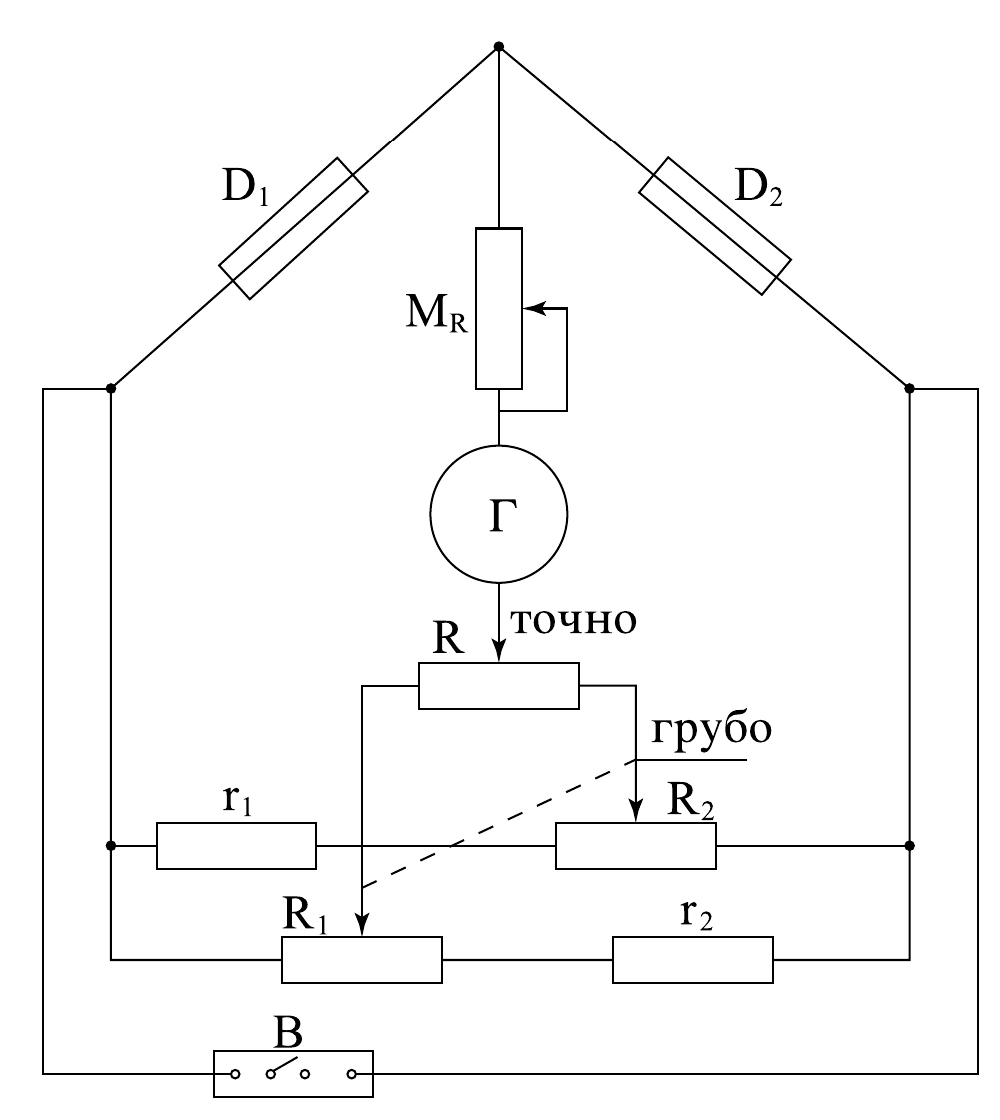
\includegraphics[scale = 0.2]{scheme2.png}
  \caption{Принципиальная схема моста.}
\end{wrapfigure}
Здесь D$_{1}$ и D$_{2}$~--- датчики теплопроводности, расположенные а сосудах $V_{1}$ и $V_{2}$. Сопротивления $R_{1}$, $R_{2}$ и $R$ служат для установки прибора на нуль (балансировка моста). В одну из диагоналей моста включен гальванометр, к другой подключается небольшое постоянное напряжение. В одну из диагоналей моста включен гальванометр, к другой подключается небольшое постоянное напряжение. Мост балансируется при заполнении сосудов (и датчиков) одной и той же смесью. При заполнении сосудов свесями различного состава возникает <<разбаланс>> моста, зависящий от разности концентраций.\\
Зависимости теплопроводности смеси газов от ее состава, вообще говоря, довольно сложна, но при достаточно малых изменениях концентрации ($\sim 15\%$) величину тока можно считать прямо пропорциональной разности концентраций (в этом случае поправка не превышает $0,5\%$).\\
В процессе диффузии разность концентраций убывает по закону~\ref{eq6}. По тому же закону изменяются и показания гальванометра.
\begin{equation}
  V = V_{0} e^{-t/\tau},
\end{equation}
где $V$~--- напряжение, показываемое гальванометром в текущий момент времени, $V_{0}$~--- показываемое в начальный момент времени.
\section{Результаты измерений и обработка данных.}
\subsection{Первая серия измерений ($P_{1} = 38,8\ торр$).}
Очистим установку от всех газов, которые там есть. Затем запускаем воздух при давлении $P_{1} = 38,8\ торр$. В сосуд $V_{1}$ к воздуху добавим некоторое количество гелия. Теперь уравняем давления, открыв краны К$_{1}$ и К$_{2}$. Диффузия здесь будет происходить довольно медленно, и к тому в нашей работе исследутся закон, описывающий изменение разницы давлений.\\
Теперь откроем кран К$_{3}$ и начнем измерения. Результаты представленнны в таблицах~\ref{table:tab1.1} и \ref{table:tab1.2}.
По результатам измерений построим график.
\begin{figure}[h!]\label{fig:img3}
  \centering
  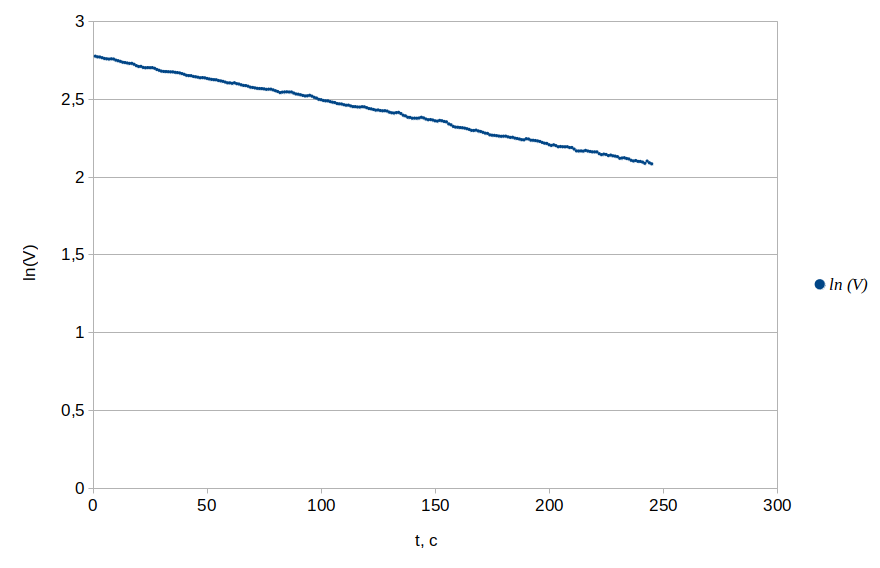
\includegraphics[scale = 0.4125]{graph1.png}
  \caption{График результатов измерения зависимости $V$ от времени в первой серии измерений ($P = 38,8\ торр$).}
\end{figure}
\subsection{Вторая серия измерений ($P_{2} = 83,5\ торр$).}
Повторим измерения для давления $P_{2} = 83,5\ торр$. Результаты представленнны в таблицe~2.
По результатам измерений построим график.
\begin{figure}[h!]\label{fig:img4}
  \centering
  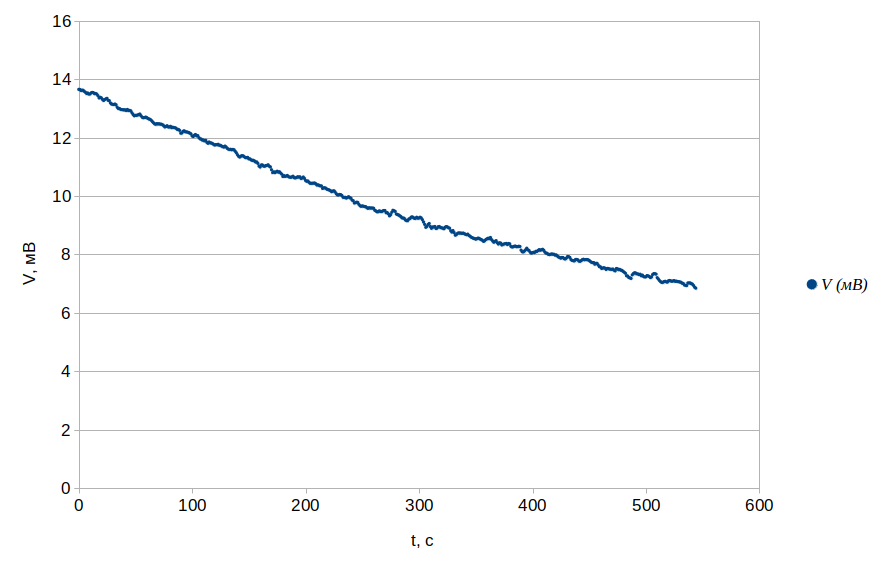
\includegraphics[scale = 0.4125]{graph2.png}
  \caption{График результатов измерения зависимости $V$ от времени во второй серии измерений ($P = 83,5\ торр$).}
\end{figure}
\subsection{Вторая серия измерений ($P_{3} = 121,3\ торр$).}
Повторим измерения для давления $P_{3} = 121,3\ торр$. Результаты представленнны в таблицe~2.
По результатам измерений построим график.
\begin{figure}[h!]\label{fig:img4}
  \centering
  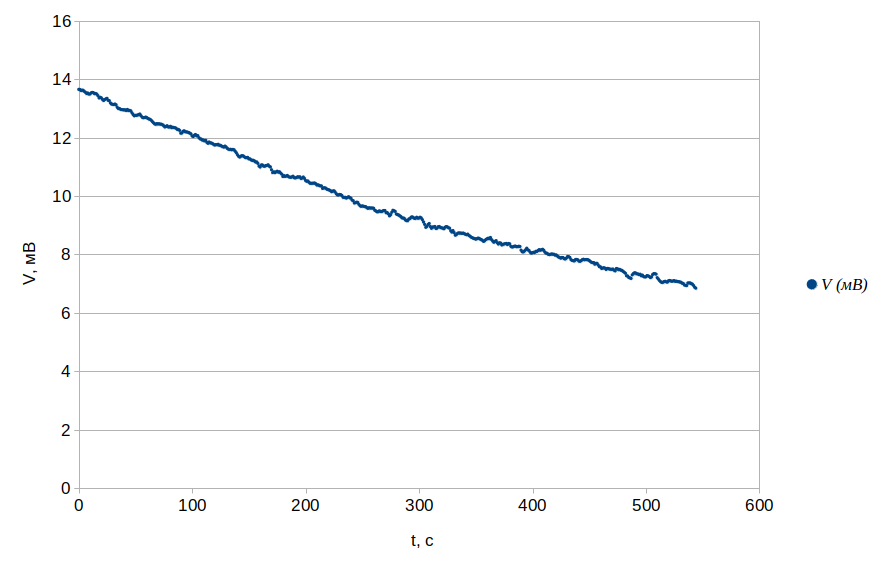
\includegraphics[scale = 0.4125]{graph2.png}
  \caption{График результатов измерения зависимости $V$ от времени в третьей серии измерений ($P = 121,3\ торр$).}
\end{figure}
\subsection{Вторая серия измерений ($P_{4} = 164,5\ торр$).}
Повторим измерения для давления $P_{3} = 164,5\ торр$. Результаты представленнны в таблицe~2.
По результатам измерений построим график.
\begin{figure}[h!]\label{fig:img4}
  \centering
  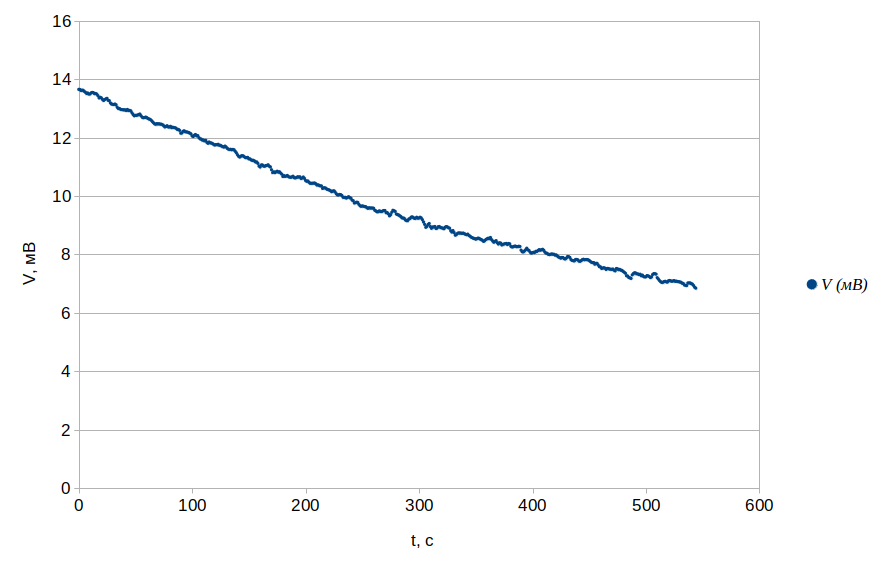
\includegraphics[scale = 0.4125]{graph2.png}
  \caption{График результатов измерения зависимости $V$ от времени в третьей серии измерений ($P = 164,5\ торр$).}
\end{figure}
\end{document}
